\documentclass[11pt,compress,t,notes=noshow, xcolor=table]{beamer}
\usepackage[]{graphicx}\usepackage[]{color}
% maxwidth is the original width if it is less than linewidth
% otherwise use linewidth (to make sure the graphics do not exceed the margin)
\makeatletter
\def\maxwidth{ %
  \ifdim\Gin@nat@width>\linewidth
    \linewidth
  \else
    \Gin@nat@width
  \fi
}
\makeatother

\definecolor{fgcolor}{rgb}{0.345, 0.345, 0.345}
\newcommand{\hlnum}[1]{\textcolor[rgb]{0.686,0.059,0.569}{#1}}%
\newcommand{\hlstr}[1]{\textcolor[rgb]{0.192,0.494,0.8}{#1}}%
\newcommand{\hlcom}[1]{\textcolor[rgb]{0.678,0.584,0.686}{\textit{#1}}}%
\newcommand{\hlopt}[1]{\textcolor[rgb]{0,0,0}{#1}}%
\newcommand{\hlstd}[1]{\textcolor[rgb]{0.345,0.345,0.345}{#1}}%
\newcommand{\hlkwa}[1]{\textcolor[rgb]{0.161,0.373,0.58}{\textbf{#1}}}%
\newcommand{\hlkwb}[1]{\textcolor[rgb]{0.69,0.353,0.396}{#1}}%
\newcommand{\hlkwc}[1]{\textcolor[rgb]{0.333,0.667,0.333}{#1}}%
\newcommand{\hlkwd}[1]{\textcolor[rgb]{0.737,0.353,0.396}{\textbf{#1}}}%
\let\hlipl\hlkwb

\usepackage{framed}
\makeatletter
\newenvironment{kframe}{%
 \def\at@end@of@kframe{}%
 \ifinner\ifhmode%
  \def\at@end@of@kframe{\end{minipage}}%
  \begin{minipage}{\columnwidth}%
 \fi\fi%
 \def\FrameCommand##1{\hskip\@totalleftmargin \hskip-\fboxsep
 \colorbox{shadecolor}{##1}\hskip-\fboxsep
     % There is no \\@totalrightmargin, so:
     \hskip-\linewidth \hskip-\@totalleftmargin \hskip\columnwidth}%
 \MakeFramed {\advance\hsize-\width
   \@totalleftmargin\z@ \linewidth\hsize
   \@setminipage}}%
 {\par\unskip\endMakeFramed%
 \at@end@of@kframe}
\makeatother

\definecolor{shadecolor}{rgb}{.97, .97, .97}
\definecolor{messagecolor}{rgb}{0, 0, 0}
\definecolor{warningcolor}{rgb}{1, 0, 1}
\definecolor{errorcolor}{rgb}{1, 0, 0}
\newenvironment{knitrout}{}{} % an empty environment to be redefined in TeX

\usepackage{alltt}
\newcommand{\SweaveOpts}[1]{}  % do not interfere with LaTeX
\newcommand{\SweaveInput}[1]{} % because they are not real TeX commands
\newcommand{\Sexpr}[1]{}       % will only be parsed by R
\newcommand{\xmark}{\ding{55}}%


\usepackage[english]{babel}
\usepackage[utf8]{inputenc}

\usepackage{dsfont}
\usepackage{verbatim}
\usepackage{amsmath}
\usepackage{amsfonts}
\usepackage{amssymb}
\usepackage{bm}
\usepackage{csquotes}
\usepackage{multirow}
\usepackage{longtable}
\usepackage{booktabs}
\usepackage{enumerate}
\usepackage[absolute,overlay]{textpos}
\usepackage{psfrag}
\usepackage{algorithm}
\usepackage{algpseudocode}
\usepackage{eqnarray}
\usepackage{arydshln}
\usepackage{tabularx}
\usepackage{placeins}
\usepackage{tikz}
\usepackage{setspace}
\usepackage{colortbl}
\usepackage{mathtools}
\usepackage{wrapfig}
\usepackage{bm}
\usepackage{amsmath}
\usepackage{pifont}
\usepackage{xcolor} %colored math symbols

\usetikzlibrary{shapes,arrows,automata,positioning,calc,chains,trees, shadows}
\tikzset{
  %Define standard arrow tip
  >=stealth',
  %Define style for boxes
  punkt/.style={
    rectangle,
    rounded corners,
    draw=black, very thick,
    text width=6.5em,
    minimum height=2em,
    text centered},
  % Define arrow style
  pil/.style={
    ->,
    thick,
    shorten <=2pt,
    shorten >=2pt,}
}

\usepackage{subfig}

% Defines macros and environments
\usepackage{../../style/lmu-lecture}


\let\code=\texttt
\let\proglang=\textsf

\setkeys{Gin}{width=0.9\textwidth}

\setbeamertemplate{frametitle}{\expandafter\uppercase\expandafter\insertframetitle}

\usepackage{bbm}
% basic latex stuff
\newcommand{\pkg}[1]{{\fontseries{b}\selectfont #1}} %fontstyle for R packages
\newcommand{\lz}{\vspace{0.5cm}} %vertical space
\newcommand{\dlz}{\vspace{1cm}} %double vertical space
\newcommand{\oneliner}[1] % Oneliner for important statements
{\begin{block}{}\begin{center}\begin{Large}#1\end{Large}\end{center}\end{block}}


%new environments
\newenvironment{vbframe}  %frame with breaks and verbatim
{
 \begin{frame}[containsverbatim,allowframebreaks]
}
{
\end{frame}
}

\newenvironment{vframe}  %frame with verbatim without breaks (to avoid numbering one slided frames)
{
 \begin{frame}[containsverbatim]
}
{
\end{frame}
}

\newenvironment{blocki}[1]   % itemize block
{
 \begin{block}{#1}\begin{itemize}
}
{
\end{itemize}\end{block}
}

\newenvironment{fragileframe}[2]{  %fragile frame with framebreaks
\begin{frame}[allowframebreaks, fragile, environment = fragileframe]
\frametitle{#1}
#2}
{\end{frame}}


\newcommand{\myframe}[2]{  %short for frame with framebreaks
\begin{frame}[allowframebreaks]
\frametitle{#1}
#2
\end{frame}}

\newcommand{\remark}[1]{
  \textbf{Remark:} #1
}


\newenvironment{deleteframe}
{
\begingroup
\usebackgroundtemplate{
\includegraphics[width=\paperwidth,height=\paperheight]{../style/color/red.png}}
 \begin{frame}
}
{
\end{frame}
\endgroup
}
\newenvironment{simplifyframe}
{
\begingroup
\usebackgroundtemplate{
\includegraphics[width=\paperwidth,height=\paperheight]{../style/color/yellow.png}}
 \begin{frame}
}
{
\end{frame}
\endgroup
}\newenvironment{draftframe}
{
\begingroup
\usebackgroundtemplate{
\includegraphics[width=\paperwidth,height=\paperheight]{../style/color/green.jpg}}
 \begin{frame}
}
{
\end{frame}
\endgroup
}
% https://tex.stackexchange.com/a/261480: textcolor that works in mathmode
\makeatletter
\renewcommand*{\@textcolor}[3]{%
  \protect\leavevmode
  \begingroup
    \color#1{#2}#3%
  \endgroup
}
\makeatother


\input{../../latex-math/basic-math}
\input{../../latex-math/basic-ml}
\input{../../latex-math/ml-nn}

\newcommand{\titlefigure}{figure/deepnet_one.png}
\newcommand{\learninggoals}{
  \item Architectures of deep neural networks
  \item Deep neural networks as  chained functions
  %\item  ...
}

\title{Deep Learning}
\date{}

\begin{document}

\lecturechapter{MLP -- Multi-Layer Feedforward Neural Networks}
\lecture{Deep Learning}


%\section{Multi-Layer Feedforward Neural Networks}
%%%%%%%%%%%%%%%%%%%%%%%%%%%%%%%%%%%%%%%%%%%%%%%%%%%%%%%%%%%%%%%%%%

\begin{vbframe}{Feedforward neural networks}
\begin{itemize}
\vspace{15mm}
\item We will now extend the model class once again, such that we allow an arbitrary amount $l$ of hidden layers.
\vspace{5mm}
\item The general term for this model class is (multi-layer) \textbf{feedforward networks} (inputs are passed through the network from left to right, no feedback-loops are allowed)
\end{itemize}
\framebreak
%%%%%%%%%%%%%%%%%%%%%%%%%%%%%%%%%%%%%%%%%%%%%%%%%%%%%%%%%%%%%%%%%%

\begin{itemize}
\item We can characterize those models by the following chain structure: $$\fx = \tau \circ \phi \circ \sigma^{(l)} \circ \phi^{(l)} \circ \sigma^{(l-1)} \circ \phi^{(l-1)} \circ \ldots \circ \sigma^{(1)} \circ \phi^{(1)}$$ where $\sigma^{(i)}$ and $\phi^{(i)}$ are the activation function and the weighted sum of hidden layer $i$, respectively. $\tau$ and $\phi$ are the corresponding components of the output layer.
\vspace{5mm}
\item Each hidden layer has: 
\begin{itemize}
\vspace{2mm}
\item an associated weight matrix $\Wmat^{(i)}$, bias $\biasb^{(i)}$, and activations $\hidz^{(i)}$ for $i \in \{ 1 \ldots l\}$.
\vspace{2mm}
\item $\hidz^{(i)} = \sigma^{(i)}(\phi^{(i)}) = \sigma^{(i)}(\Wmat^{(i)T}\hidz^{(i - 1)} + \biasb^{(i)})$ , where $\hidz^{(0)} = \xv$.
\end{itemize}
\vspace{5mm}
\item Again, without non-linear activations in the hidden layers, the network can only learn linear decision boundaries.
  \end{itemize}
\framebreak
%%%%%%%%%%%%%%%%%%%%%%%%%%%%%%%%%%%%%%%%%%%%%%%%%%%%%%%%%%%%%%%%%%

\lz
\begin{figure}
\centering
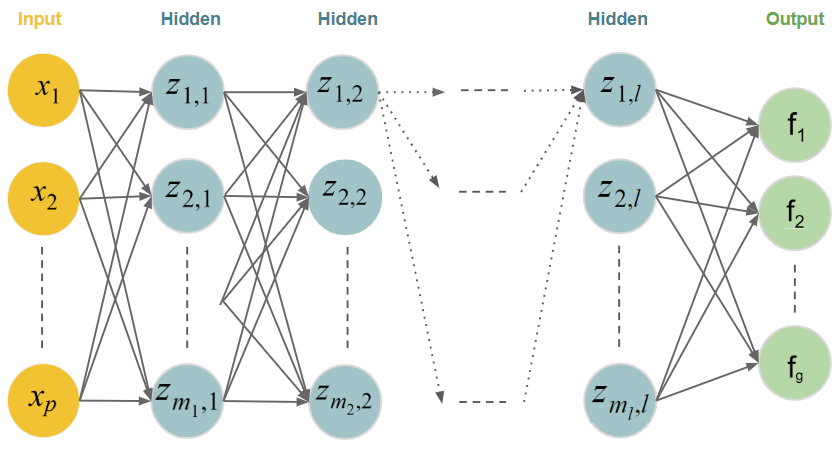
\includegraphics[width=10.5cm]{figure/deepneuralnet_new.png}
\caption{Structure of a deep neural network with $l$ hidden layers (bias terms omitted).}
  \end{figure}
\end{vbframe}  
%%%%%%%%%%%%%%%%%%%%%%%%%%%%%%%%%%%%%%%%%%%%%%%%%%%%%%%%%%%%%%%%%%

\begin{frame} {Feedforward neural networks: Example}
\begin{figure}
\centering
\only<1>{\scalebox{0.95}{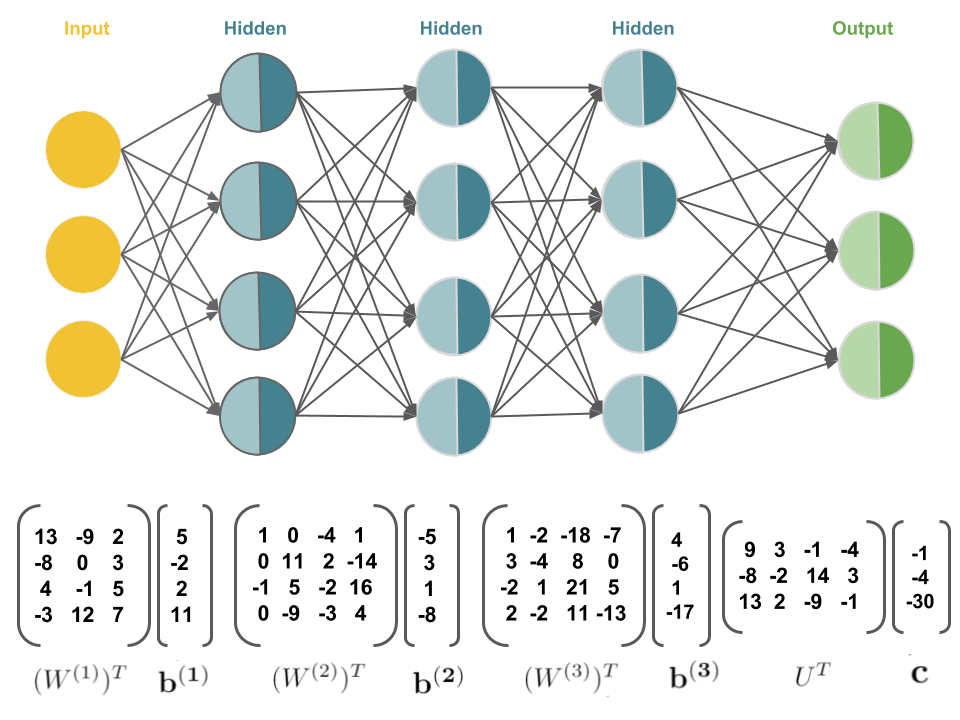
\includegraphics{figure/deepnet_one.png}}}
\only<2>{\scalebox{0.95}{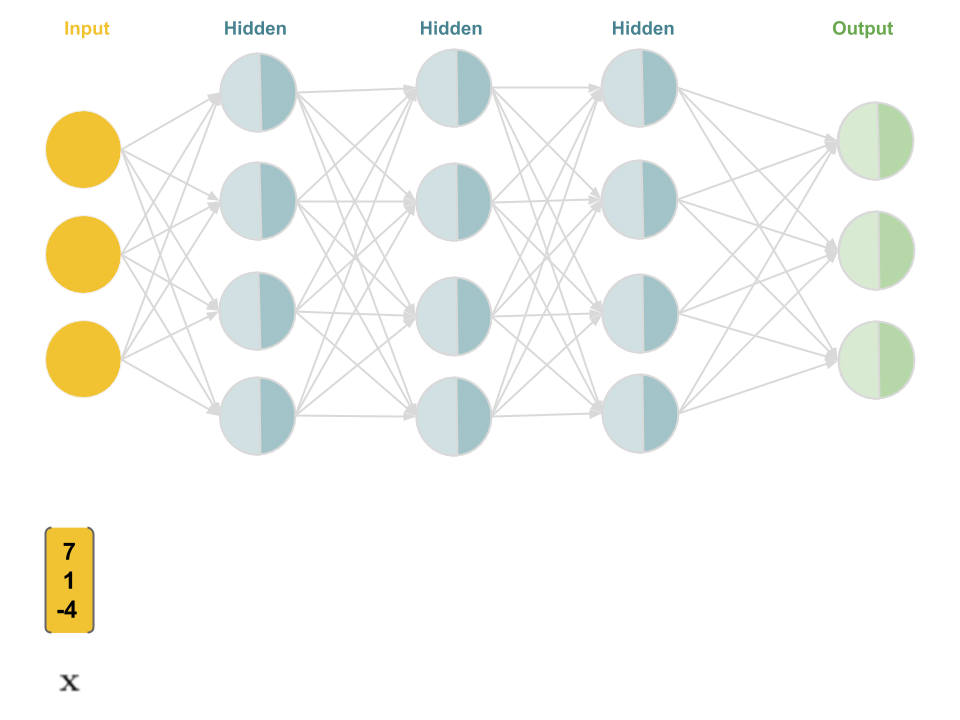
\includegraphics{figure/deepnet_two.png}}}
\only<3>{\scalebox{0.95}{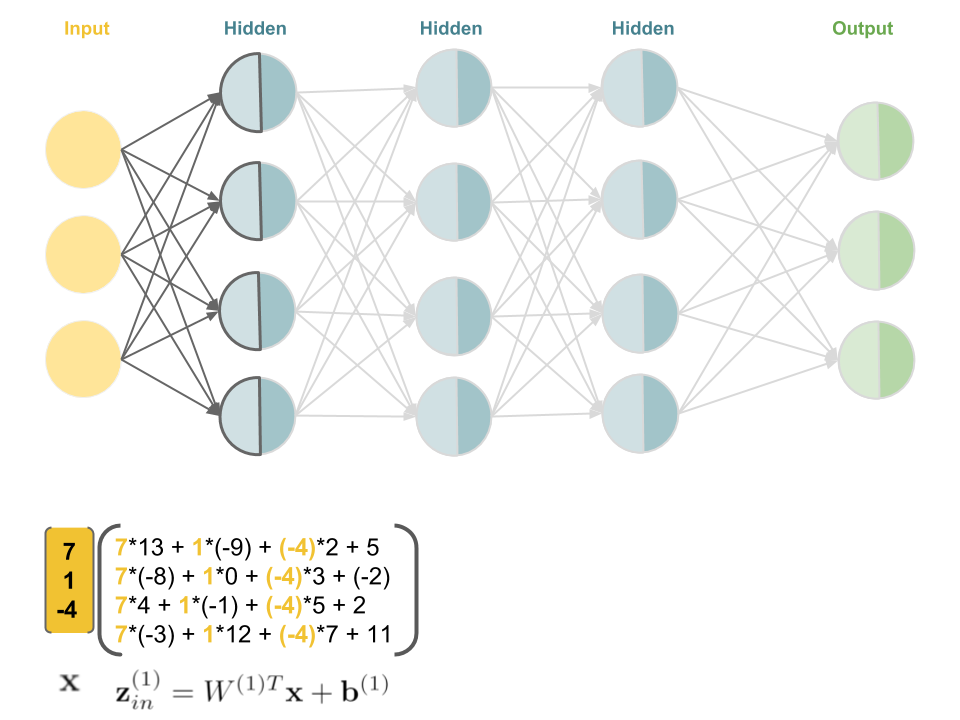
\includegraphics{figure/deepnet_three.png}}}
\only<4>{\scalebox{0.95}{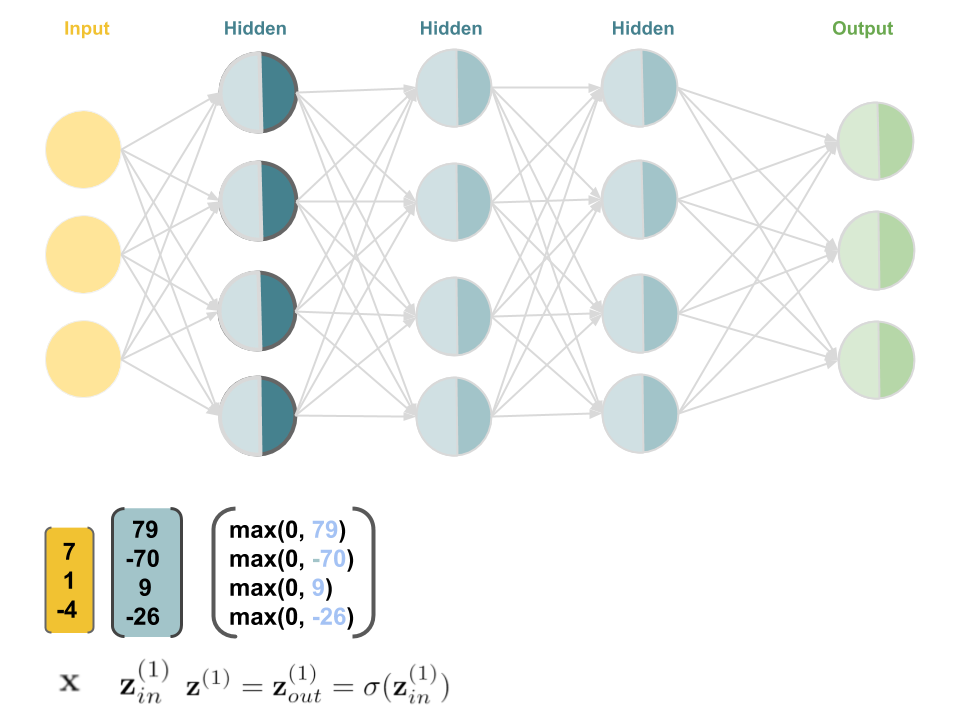
\includegraphics{figure/deepnet_four.png}}}
\only<5>{\scalebox{0.95}{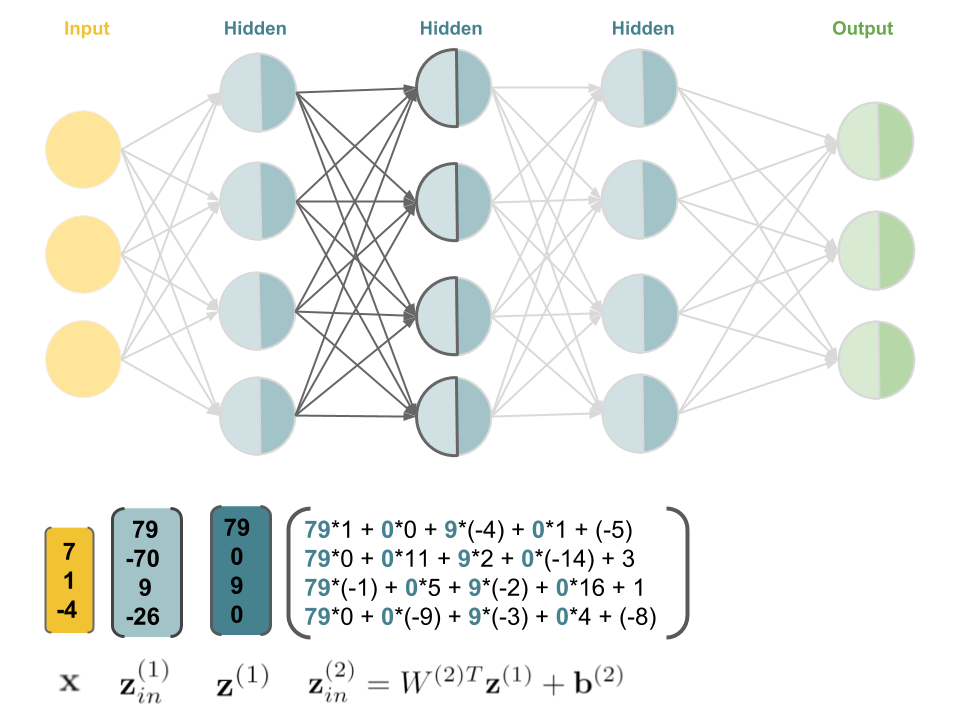
\includegraphics{figure/deepnet_five.png}}}
\only<6>{\scalebox{0.95}{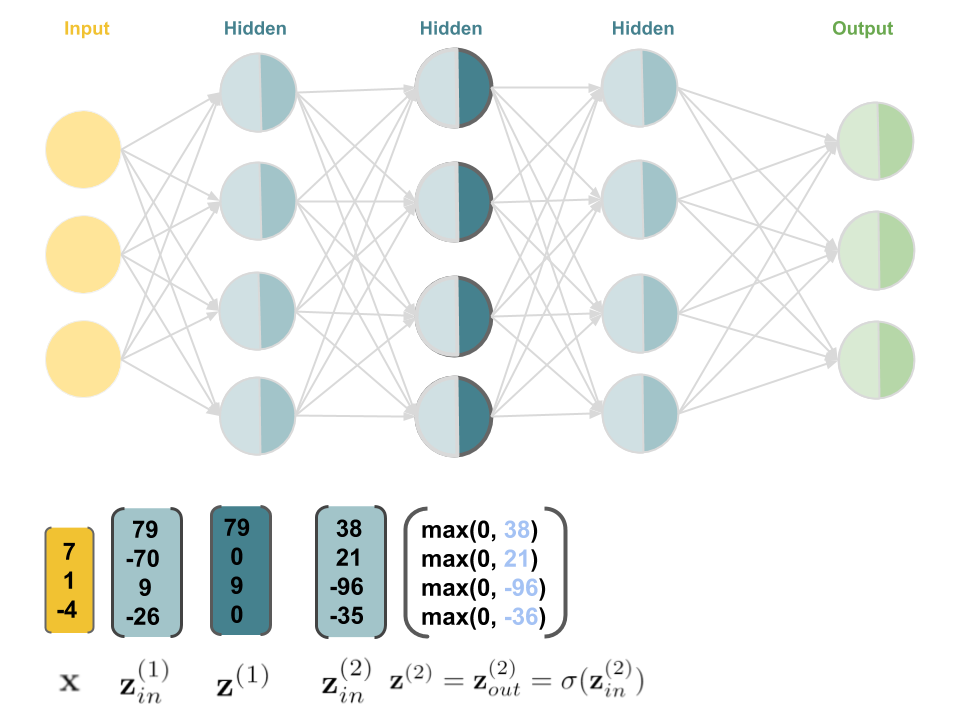
\includegraphics{figure/deepnet_six.png}}}
\only<7>{\scalebox{0.95}{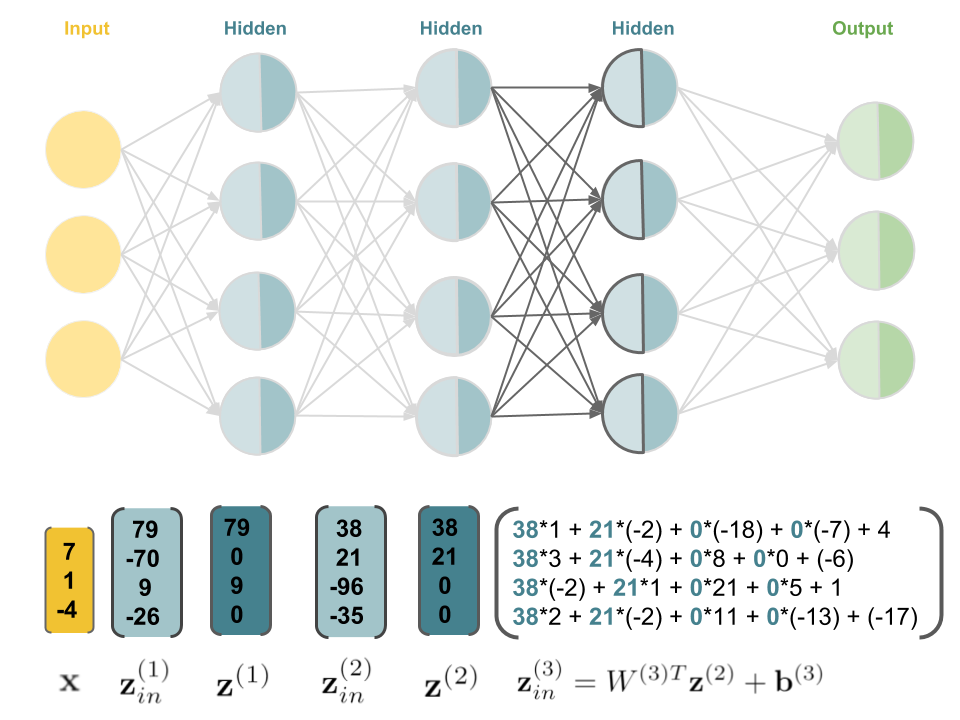
\includegraphics{figure/deepnet_seven.png}}}
\only<8>{\scalebox{0.95}{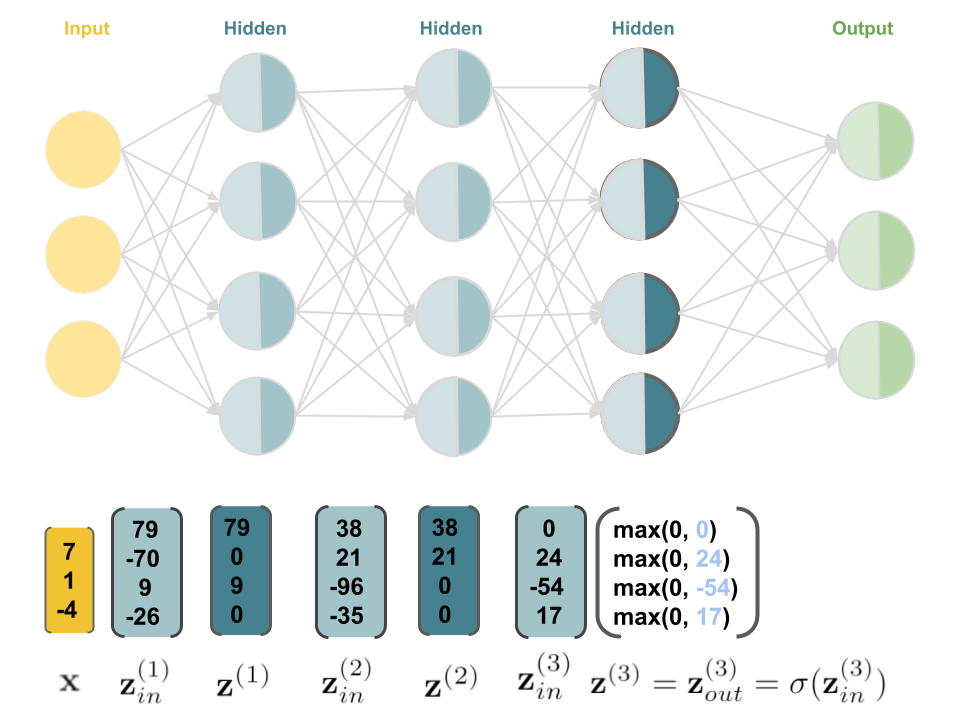
\includegraphics{figure/deepnet_eight.png}}}
\only<9>{\scalebox{0.95}{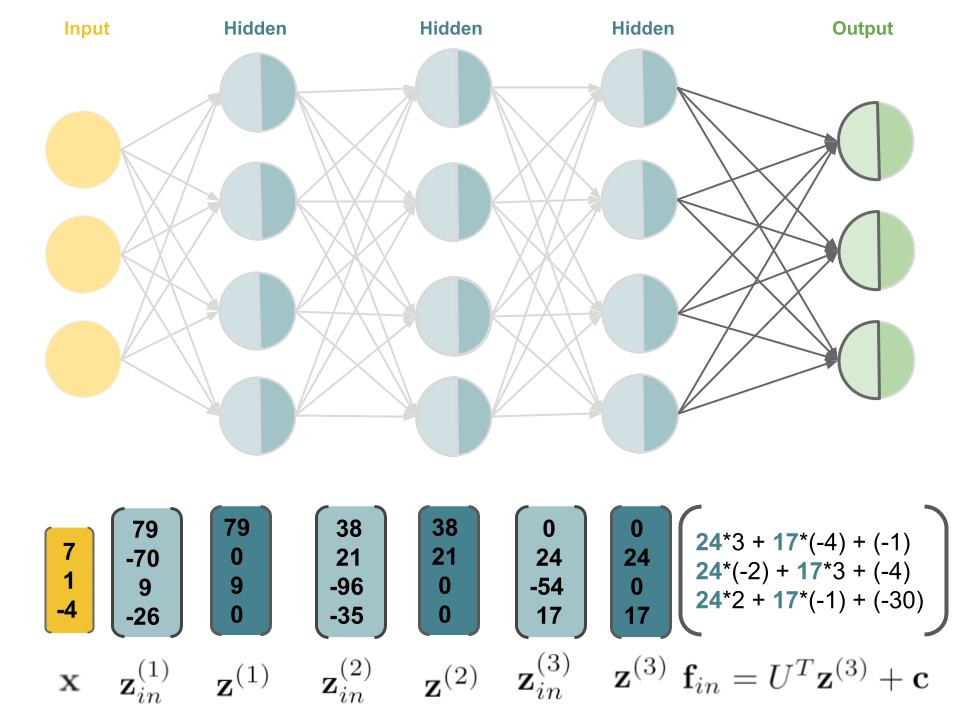
\includegraphics{figure/deepnet_nine.png}}}
\only<10>{\scalebox{0.95}{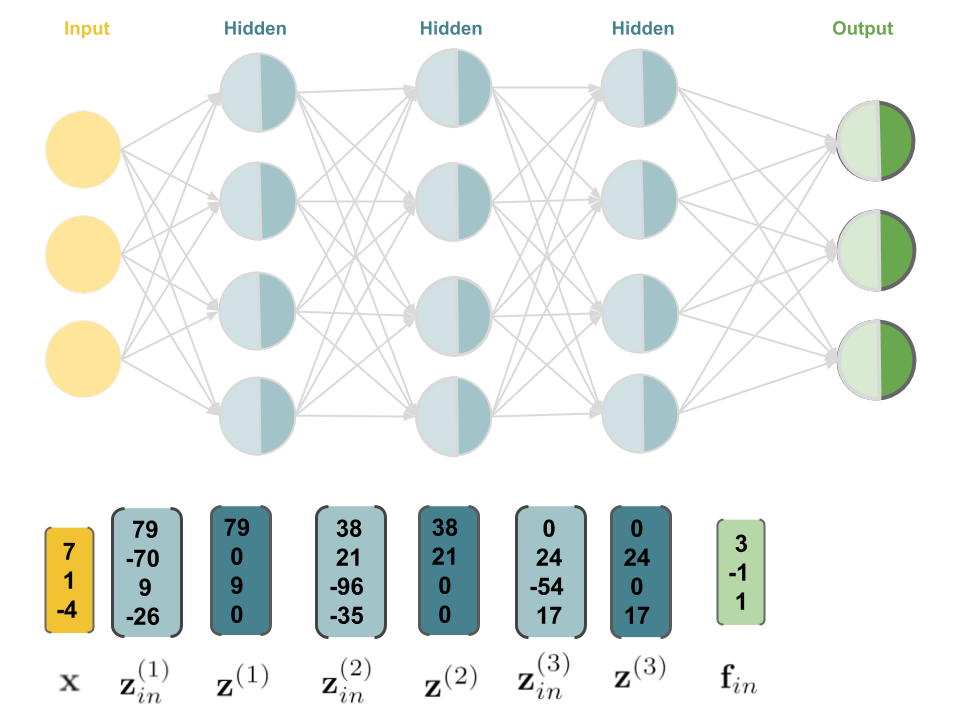
\includegraphics{figure/deepnet_ten.png}}}
\only<11>{\scalebox{0.95}{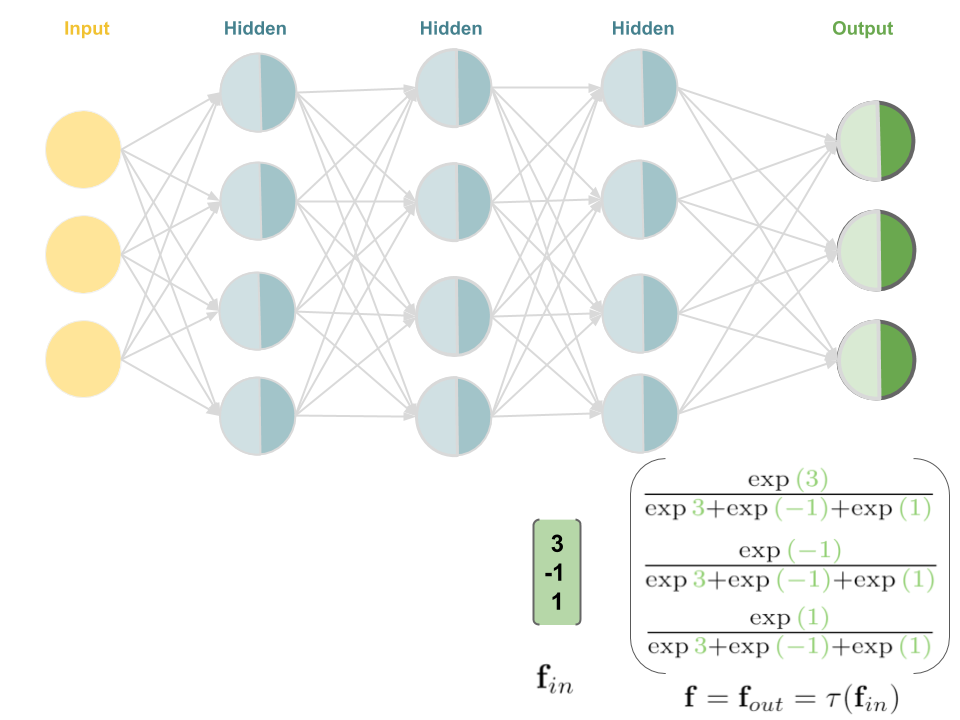
\includegraphics{figure/deepnet_eleven.png}}}
\only<12>{\scalebox{0.95}{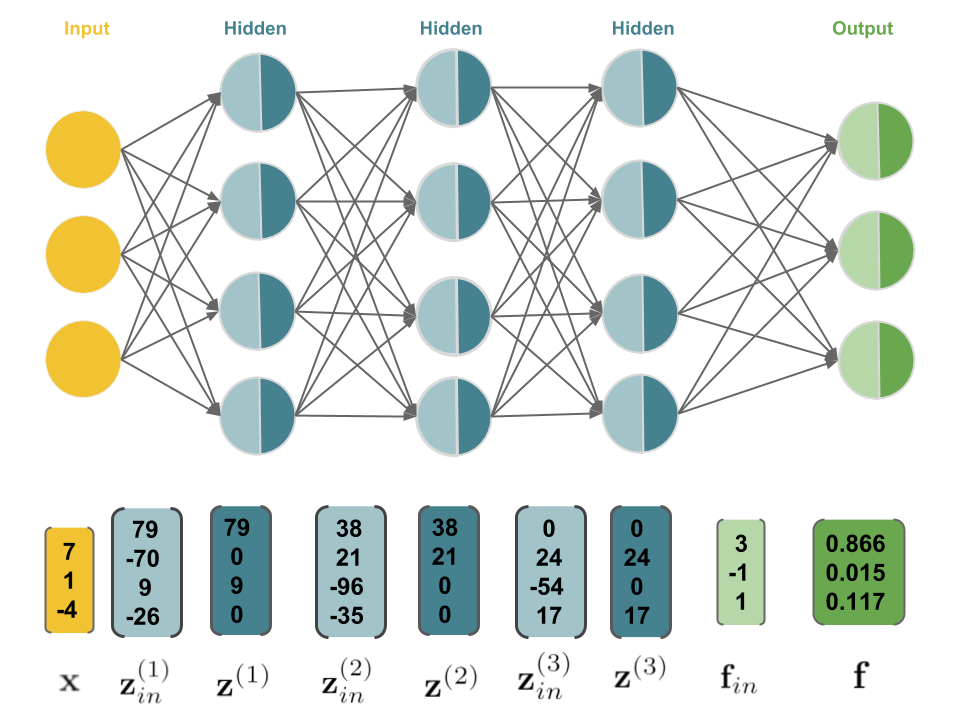
\includegraphics{figure/deepnet_twelve.png}}}
\end{figure}
\end{frame}
%%%%%%%%%%%%%%%%%%%%%%%%%%%%%%%%%%%%%%%%%%%%%%%%%%%%%%%%%%%%%%%%%%

\begin{vbframe}{Why add more layers?}
\begin{itemize}
\item Multiple layers allow for the extraction of more and more abstract
representations.
%\lz
\item Each layer in a feed-forward neural network adds its own degree of non-lnearity to the model.
\end{itemize}
%\lz
\begin{figure}
\centering
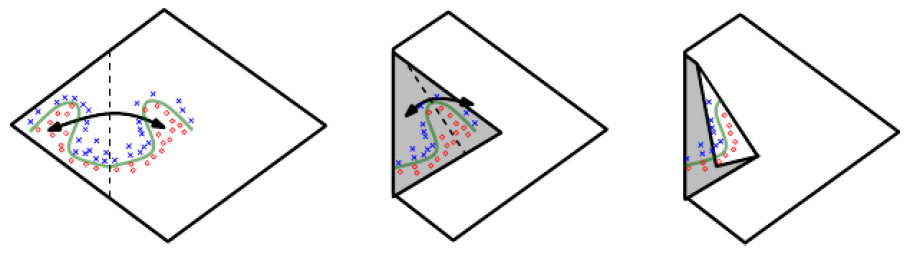
\includegraphics[width=10.5cm]{figure/folding}
\caption{An intuitive, geometric explanation of the exponential advantage of deeper networks formally (Mont\'{u}far et al., 2014).}
\end{figure}
\end{vbframe}
%%%%%%%%%%%%%%}%%%%%%%%%%%%%%%%%%%%%%%%%%%%%%%%%%%%%%%%%%%%%%%%%%%%%

\begin{vbframe}{Deep neural networks}

Neural networks today can have %dozens or even 
hundreds of hidden layers. The greater the number of layers, the "deeper" the network. Historically %, however, 
DNNs were very challenging to train and not popular until the late '00s for several reasons:
\lz
\begin{itemize}
\item %For one thing, the 
The use of sigmoid activations (e.g., logistic sigmoid and tanh) significantly slowed down training due to a phenomenon known as \enquote{vanishing gradients}. The introduction of the ReLU activation largely solved this problem.
\item Training DNNs on CPUs was too slow to be practical. Switching over to GPUs cut down training time by more than an order of magnitude.
\item When dataset sizes are small, other models (such as SVMs) and techniques (such as feature engineering) often outperform them. 
\end{itemize}
\framebreak
%%%%%%%%%%%%%%%%%%%%%%%%%%%%%%%%%%%%%%%%%%%%%%%%%%%%%%%%%%%%%%%%%%
\begin{itemize}
\item The availability of large datasets and novel architectures that are capable of handling even complex tensor-shaped data (e.g. CNNs for image data), faster hardware, and better optimization and regularization methods made it feasible to successfully implement deep neural networks.% in the last decade.
\lz

\item An increase in depth often translates to an increase in performance on a given task. State-of-the-art neural networks, however, are much more sophisticated than the simple architectures we have encountered so far.

\lz
%\item 
\end{itemize}
The term "\textbf{deep learning}" encompasses all of these developments and refers to the field as a whole.
\end{vbframe}
%%%%%%%%%%%%%%%%%%%%%%%%%%%%%%%%%%%%%%%%%%%%%%%%%%%%%%%%%%%%%%%%%%
%%%%%%%%%%%%%%%%%%%%%%%%%%%%%%%%%%%%%%%%%%%%%%%%%%%%%%%%%%%%%%%%%%
%%%%%%%%%%%%%%%%%%          REFERENCES          %%%%%%%%%%%%%%%%%%
%%%%%%%%%%%%%%%%%%%%%%%%%%%%%%%%%%%%%%%%%%%%%%%%%%%%%%%%%%%%%%%%%%
\begin{vbframe}
\frametitle{References}
\footnotesize{
\begin{thebibliography}{99}
%%%%%%%%%%%%%%%%%%%%%%%%%%%%%%%%%%
\bibitem[(Mont\'{u}far et al., 2014)]{1} Mont\'{u}farr, G., Pascanu, R., Cho, K., \& Bengio, Y. (2014). \textit{On the Number of Linear Regions of Deep Neural Networks}. 
\end{thebibliography}
}
\end{vbframe}
\endlecture
\end{document}